%%
%% This is file `mcmthesis-demo.tex',
%% generated with the docstrip utility.
%%
%% The original source files were:
%%
%% mcmthesis.dtx  (with options: `demo')
%% 
%% -----------------------------------
%% 
%% This is a generated file.
%% 
%% Copyright (C)
%%     2010 -- 2015 by Zhaoli Wang
%%     2014 -- 2016 by Liam Huang
%% 
%% This work may be distributed and/or modified under the
%% conditions of the LaTeX Project Public License, either version 1.3
%% of this license or (at your option) any later version.
%% The latest version of this license is in
%%   http://www.latex-project.org/lppl.txt
%% and version 1.3 or later is part of all distributions of LaTeX
%% version 2005/12/01 or later.
%% 
%% This work has the LPPL maintenance status `maintained'.
%% 
%% The Current Maintainer of this work is Liam Huang.
%% 
\documentclass{mcmthesis}
\mcmsetup{CTeX = false,   % 使用 CTeX 套装时,设置为 true
        tcn = 0000, problem = A,
        sheet = true, titleinsheet = true, keywordsinsheet = true,
        titlepage = true, abstract = true}
\usepackage{palatino}
\usepackage{lipsum}
\title{The \LaTeX{} Template for MCM Version \MCMversion}
\author{\small \href{http://www.latexstudio.net/}
  {
\includegraphics[width=7cm]{mcmthesis-logo}}}
\date{\today}
\begin{document}
\begin{abstract}
\lipsum[1]
\begin{keywords}
keyword1; keyword2
\end{keywords}
\end{abstract}
\maketitle
\section{Introduction}
\subsection{Problem Background}
With the continuous development of Internet technology, its influence has permeated every aspect of life. Internet finance has come into being. Compared with traditional finance, Internet finance has the advantages of favoring people. For example, it achieves faster business processing speed, breaks the time and space constraints, provides faster and more convenient financial services and brings better user experience Service experience. However, at the same time, the risks it brings are becoming more and more obvious. For example, credit risk and user fraud, in this context, a set of perfect and effective credit scoring system is particularly important.\\

\subsection{Our Work}
Credit scoring is based on customer credit history data, using a certain credit score model, get different grades of credit scores. Depending on the customer's credit score, the creditor can analyze the customer's likelihood of repaying on time. Although creditors can also get the result of such analysis by analyzing the customer's credit history, the use of credit scores is faster, more objective, and more consistent.\\
\newline
Given that Logistic regression algorithms are often used in today's commercial credit scoring models, we mainly try this algorithm and decision tree algorithms to train, focusing on data cleaning and variable selection and construction. Some of the choices for variable selection are mainly the screening of credit scores commonly used in the industry. For the given data, we mainly do the following thinking:\\
\begin{itemize}
\item Which of these customer data sets is unusable.
\item What is the ratio between good and bad customers, how to deal with imbalances.
\item The amount of data itself is not large, how to make the model more fully trained.
\item How to evaluate data to promote model training.
\item Some of the data to do some conversion, making it more suitable for training.
\item Training algorithm itself parameters should be adjusted to the problem.
\end{itemize}
The back of the content will be reflected above.\\

\section{Assumptions}
\begin{itemize}
\item Assume that the historical business data of the lender is stable and trustworthy
\item Assume the default is not affected by emergencies
\item Assume that all borrowers have good credit history before
\end{itemize}

\section{Data Processing}
\subsection{Data Screening}
The amount of data is large, so our priority is to filter the data based on its completeness and validity.\\
First, we screen the data of 30,000 historical business data provided by the lender:\\
\begin{itemize}
\item Since tag attributes are crucial and can not be completed, we delete all business data that did not indicate a default.
\item In the analysis of the attributes, we found that there are a large number of missing attributes of AGENT and salary level in the data, in which the salary level can be complemented because it is a numerical attribute with continuous meaning. For AGENT, because it is text type data and Did not find it related to other attributes, so we choose to delete AGENT this attribute.
\end{itemize}

\subsection{Data Merging}
\begin{itemize}
\item when processing the data we found that the education level variables, there are college and below, junior high school and junior high school, the four classification of repeated phenomena, which are repeated graduate, doctoral and master's degree and more than three kinds of classification, so we will and specialist and below master degree or above and two classification.
\item at the same time, we found that two kinds of definitions of divorce and divorce were duplicated in the marital status. We merged them into divorce. At the same time, we considered the semantic description of marital status. We merged the widowhood into divorce and merged the other into the unmarried.
\item for borrowing time, we provide data from January to June 2017, so we combine it into 6 categories representing 6 months to facilitate later use. .
\item for the working provinces, we divide the provinces into four large areas, the eastern, the northeast, the central and the western regions, according to the division of the sixteen regions of the Communist Party of China and the development of the provinces in the past year (Figure).
\end{itemize}

\subsection{Missing Value Processing}
2.3 Missing Value Processing

In statistics, missing data occur when no data value is stored for the variable in an observation.Missing data are a common occurrence and can have a significant effect on the conclusions that can be drawn from the data.\\
\newline
In the data we use, there is a large amount of data that is missing a salary grade variable, and we consider doing so due to the lack of a large amount of data and the variable is a numeric data with a continuous relationship. We have statistics on the available data and found that the overall data is normally distributed.\\
% 图

Then we consider that the pay scale may be influenced by the level of education and the work area, so we will analyze it on the assumption that different education levels and pay scales are different from those in the work area.\\
% pic
We found that at different levels of education, salary levels are basically normal distribution, so taking the level of compensation at different levels of education found. The proportion of high salaries at the educational level of masters and above is higher than that of other education levels. However, taking into consideration the low level of data in this level of education, The horizontal approximation is seen as a normal distribution.\\
\newline
For different workplaces, we also analyze their salary levels.\\
We also found that in all workplaces, all salary levels are normally distributed, so we conclude that the salary level in this data is normally distributed, with no educational level or work area impact.
\newline
In this regard, we take the average and mode and draw the relevant charts for a preliminary analysis.\\
% biao
We can see that the average is 3.58 and the mode is 3. Taking into consideration and facilitating our later use, we decided to set the missing value of all pay levels to 3.\\

\section{Our Model}
Based on available information, consider the current credit scoring model and the industry's interpretative requirements for credit scoring models. Our initial consideration of the model is logistic regression.
\newline
The data, the marital status can not simply use the serial number to represent, this will result in some similar marital status but the actual situation is not. The marriage attribute itself is not sequential, so we carried out One-Hot encoding. By the same token, taking into account the rough change of the academic data itself, the order of academic qualifications becomes vague, and we also carry the One-Hot code for academic qualifications. Finally, consider the province data, the province of our data is a 6-digit zip code. It is observed that the left-most 2-digit postcode represents its province, so we converted that data to obtain the customer's province code. Taking into account the large number of provinces in China, we have reviewed the relevant information and found that China is divided into four major economic regions: the eastern region, the northeast region, the central region and the western region. The main contents of economic and social development in various regions are: development in the west, rejuvenation in the northeast, rise in the middle and development in the east. Taking into account the loan, credit score and economy, we divided the provinces data:
\newline
Northeast China (Heilongjiang, Jilin, Liaoning, Hulunbeier, Xing'an League, Tongliao, Chifeng, Xilin Gol League in eastern Inner Mongolia Autonomous Region)
\newline
Middle region (Shanxi, Henan, Hubei, Hunan, Jiangxi, Anhui)
\newline
Eastern China (Beijing, Tianjin, Hebei, Shandong, Jiangsu, Shanghai, Zhejiang, Fujian, Guangdong, Hainan)
\newline
Western Region (Sichuan Province, Guangxi Zhuang Autonomous Region, Guizhou Province, Yunnan Province, Chongqing Municipality, Shaanxi Province, Gansu Province, West Inner Mongolia Autonomous Region, Ningxia Hui Autonomous Region, Xinjiang Uygur Autonomous Region, Qinghai Province and Tibet Autonomous Region)
\newline
The following is based on the first two digits of the ID card coding:
\begin{itemize}
  \item Northeast: 21,22,23
  \item Middle: 14,41,42,43,36,34
  \item East: 11,12,13,37,32,31,33,35,44,46  
  \item Western Region: 51,45,52,53,50,61,62,15,64,65,63,54
\end{itemize}

In fact, there is no order between provinces, so we once again conducted One-Hot encoding on the data.
\newline
After the above steps, the current data should be able to train. However, before training, we still need to do some characteristic engineering.
We use a method commonly used in the industry for screening based on IV values.
\newline
\newline
First introduce concepts and formulas.\\
\newline
\newline
The full name of IV is Information Value, find the value of wo first wo value, here also introduced the concept of woe.
\newline
WOE (weight of Evidence) is actually an influence on the proportion of default when a certain value is taken from an independent variable. After WOE encoding, the independent variable actually has some standardized nature, that is, each value of the independent variable Can be directly compared (between WOE), and various values ​​between different independent variables can also be directly compared by WOE. Furthermore, we can study the variation (fluctuation) of the WOE value in the independent variable and construct the contribution rate and relative importance of each independent variable in combination with the coefficients fitted by the model. In general, the larger the coefficient, the greater the variance of woe, the greater the contribution of the independent variable (similar to some variance contribution), which can also be intuitively understood.\\
To conclude, the process of independent variables (including coding and filtering) is largely based on the evaluation of the effects of univariate models when doing credit scoring models. In this evaluation process, ROC and IV examine the impact of independent variables on the target variables from different perspectives. Based on this investigation, we used the WOE value to encode the categorical independent variables so that the independent variables can be more intuitively understood The role of variables and direction, while enhancing the prediction effect.
\newline
The advantages of WOE transformation: Improve the predictive effect of the model and improve the comprehensibility of the model.
\newline
First group variables (how to say later), then for each group i, for the i group:
\[woe_i = \ln(\frac{B_i / B_T}{G_i / G_T})\eqno (1)\]

For example, if only the absolute value of woe is summed up, if some groups have a small number of A groups and a large number of B groups (obviously such a group is unreasonable), this is a small woe value of B and a large group A , Sum woe will not be small, apparently so unreasonable.

Finally, we can sort the variables according to the size of each variable IV value. The greater the IV to retain.

Take the credit scorecard modeling scenario as an example: X is the customer sample field, Y indicates whether the customer is overdue, where Y = 1 means overdue, Y = 0 means not overdue. We want to be able to use the information known to our clients to predict the probability of overdue after the customer borrows, in order to decide whether to lend.

We calculate the WOE value of each attribute field for the previous data, and then calculate the corresponding IV value based on the WOE value. IV measures the amount of information on a variable. IV can be used to represent the predictive power of a variable.

% \begin{Theorem} \label{thm:latex}
% \LaTeX
% \end{Theorem}
% \begin{Lemma} \label{thm:tex}
% \TeX .
% \end{Lemma}
% \begin{proof}
% The proof of theorem.
% \end{proof}

\subsection{Other Assumptions}
\lipsum[6]
\begin{itemize}
\item
\item
\item
\item
\end{itemize}

\lipsum[7]

\section{Analysis of the Problem}
\begin{figure}[h]
\small
\centering
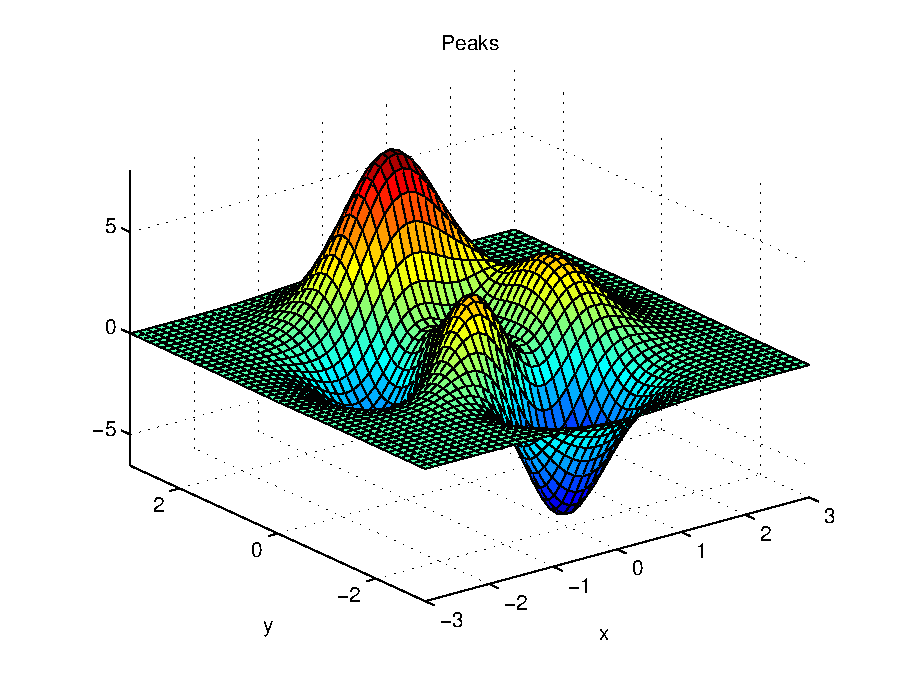
\includegraphics[width=12cm]{mcmthesis-aaa.eps}
\caption{aa} \label{fig:aa}
\end{figure}

\lipsum[8] \eqref{aa}
\begin{equation}
a^2 \label{aa}
\end{equation}

\[
  \begin{pmatrix}{*{20}c}
  {a_{11} } & {a_{12} } & {a_{13} }  \\
  {a_{21} } & {a_{22} } & {a_{23} }  \\
  {a_{31} } & {a_{32} } & {a_{33} }  \\
  \end{pmatrix}
  = \frac{{Opposite}}{{Hypotenuse}}\cos ^{ - 1} \theta \arcsin \theta
\]
\lipsum[9]

\[
  p_{j}=\begin{cases} 0,&\text{if $j$ is odd}\\
  r!\,(-1)^{j/2},&\text{if $j$ is even}
  \end{cases}
\]

\lipsum[10]

\[
  \arcsin \theta  =
  \mathop{{\int\!\!\!\!\!\int\!\!\!\!\!\int}\mkern-31.2mu
  \bigodot}\limits_\varphi
  {\mathop {\lim }\limits_{x \to \infty } \frac{{n!}}{{r!\left( {n - r}
  \right)!}}} \eqno (1)
\]

\section{Calculating and Simplifying the Model  }
\lipsum[11]

\section{The Model Results}
\lipsum[6]

\section{Validating the Model}
\lipsum[9]

\section{Conclusions}
\lipsum[6]

\section{A Summary}
\lipsum[6]

\section{Evaluate of the Mode}

\section{Strengths and weaknesses}
\lipsum[12]

\subsection{Strengths}
\begin{itemize}
\item \textbf{Applies widely}\\
This  system can be used for many types of airplanes, and it also
solves the interference during  the procedure of the boarding
airplane,as described above we can get to the  optimization
boarding time.We also know that all the service is automate.
\item \textbf{Improve the quality of the airport service}\\
Balancing the cost of the cost and the benefit, it will bring in
more convenient  for airport and passengers.It also saves many
human resources for the airline. \item \textbf{}
\end{itemize}

\begin{thebibliography}{99}
\bibitem{1} D.~E. KNUTH   The \TeX{}book  the American
Mathematical Society and Addison-Wesley
Publishing Company , 1984-1986.
\bibitem{2}Lamport, Leslie,  \LaTeX{}: `` A Document Preparation System '',
Addison-Wesley Publishing Company, 1986.
\bibitem{3}\url{http://www.latexstudio.net/}
\bibitem{4}\url{http://www.chinatex.org/}
\end{thebibliography}

\begin{appendices}

\section{First appendix}

\lipsum[13]

Here are simulation programmes we used in our model as follow.\\

\textbf{\textcolor[rgb]{0.98,0.00,0.00}{Input matlab source:}}
\lstinputlisting[language=Matlab]{./code/mcmthesis-matlab1.m}

\section{Second appendix}

some more text \textcolor[rgb]{0.98,0.00,0.00}{\textbf{Input C++ source:}}
\lstinputlisting[language=C++]{./code/mcmthesis-sudoku.cpp}

\end{appendices}
\end{document}

%% 
%% This work consists of these files mcmthesis.dtx,
%%                                   figures/ and
%%                                   code/,
%% and the derived files             mcmthesis.cls,
%%                                   mcmthesis-demo.tex,
%%                                   README,
%%                                   LICENSE,
%%                                   mcmthesis.pdf and
%%                                   mcmthesis-demo.pdf.
%%
%% End of file `mcmthesis-demo.tex'.
